\section{Deadlock recovery}
\label{sect:deadlock-exp}
MultiChain can run during normal operation into a situation
where a multiple of peers are waiting on each other as explained in section \ref{sect:deadlock}.
This could resulting in a potential deadlock.
This situation was encountered during experimentation
and the experiment shows MultiChain correctly recovering from this situation.

In the experiment a 100 megabyte file was downloaded anonymously with 2 hops.
Anonymously downloading is decribed more in the thesis report of R. Ruigrok\cite{ruigrok-anonymous}.
There are 2 Triblers instances with exit functionality and 18 instances without exit functionality.
All instances are run locally on one machine.
The instances are run in parallel,
so the fact that all instances are run on a single machine does not cause the deadlock to occur.
There is no packetloss in this experiment.

The corresponding graph of all the MultiChains of the experiment can be seen in Figure \ref{fig:deadlock-double}.
In this graph the blocks are depicted as nodes and the previous hash pointers are edges in the graph.
The nodes have added colouring to indicate extra meaning.
Green nodes are a first block in a MultiChain of a peer.
Blue nodes are a sequential block between the same previous peers.
Red nodes are half-signed blocks.

The potential scenario of two peers both waiting can be seen multiple times in the graph and are encircled.
The scenario generates a half-signed block at both peers.
Usually the peers continue collaboration and this continuation of a sequence can be seen in subsequent blocks.
In the graph a more complicated scenario can also be seen where multiple peers timeout between each other.

\begin{figure}
	\centerline{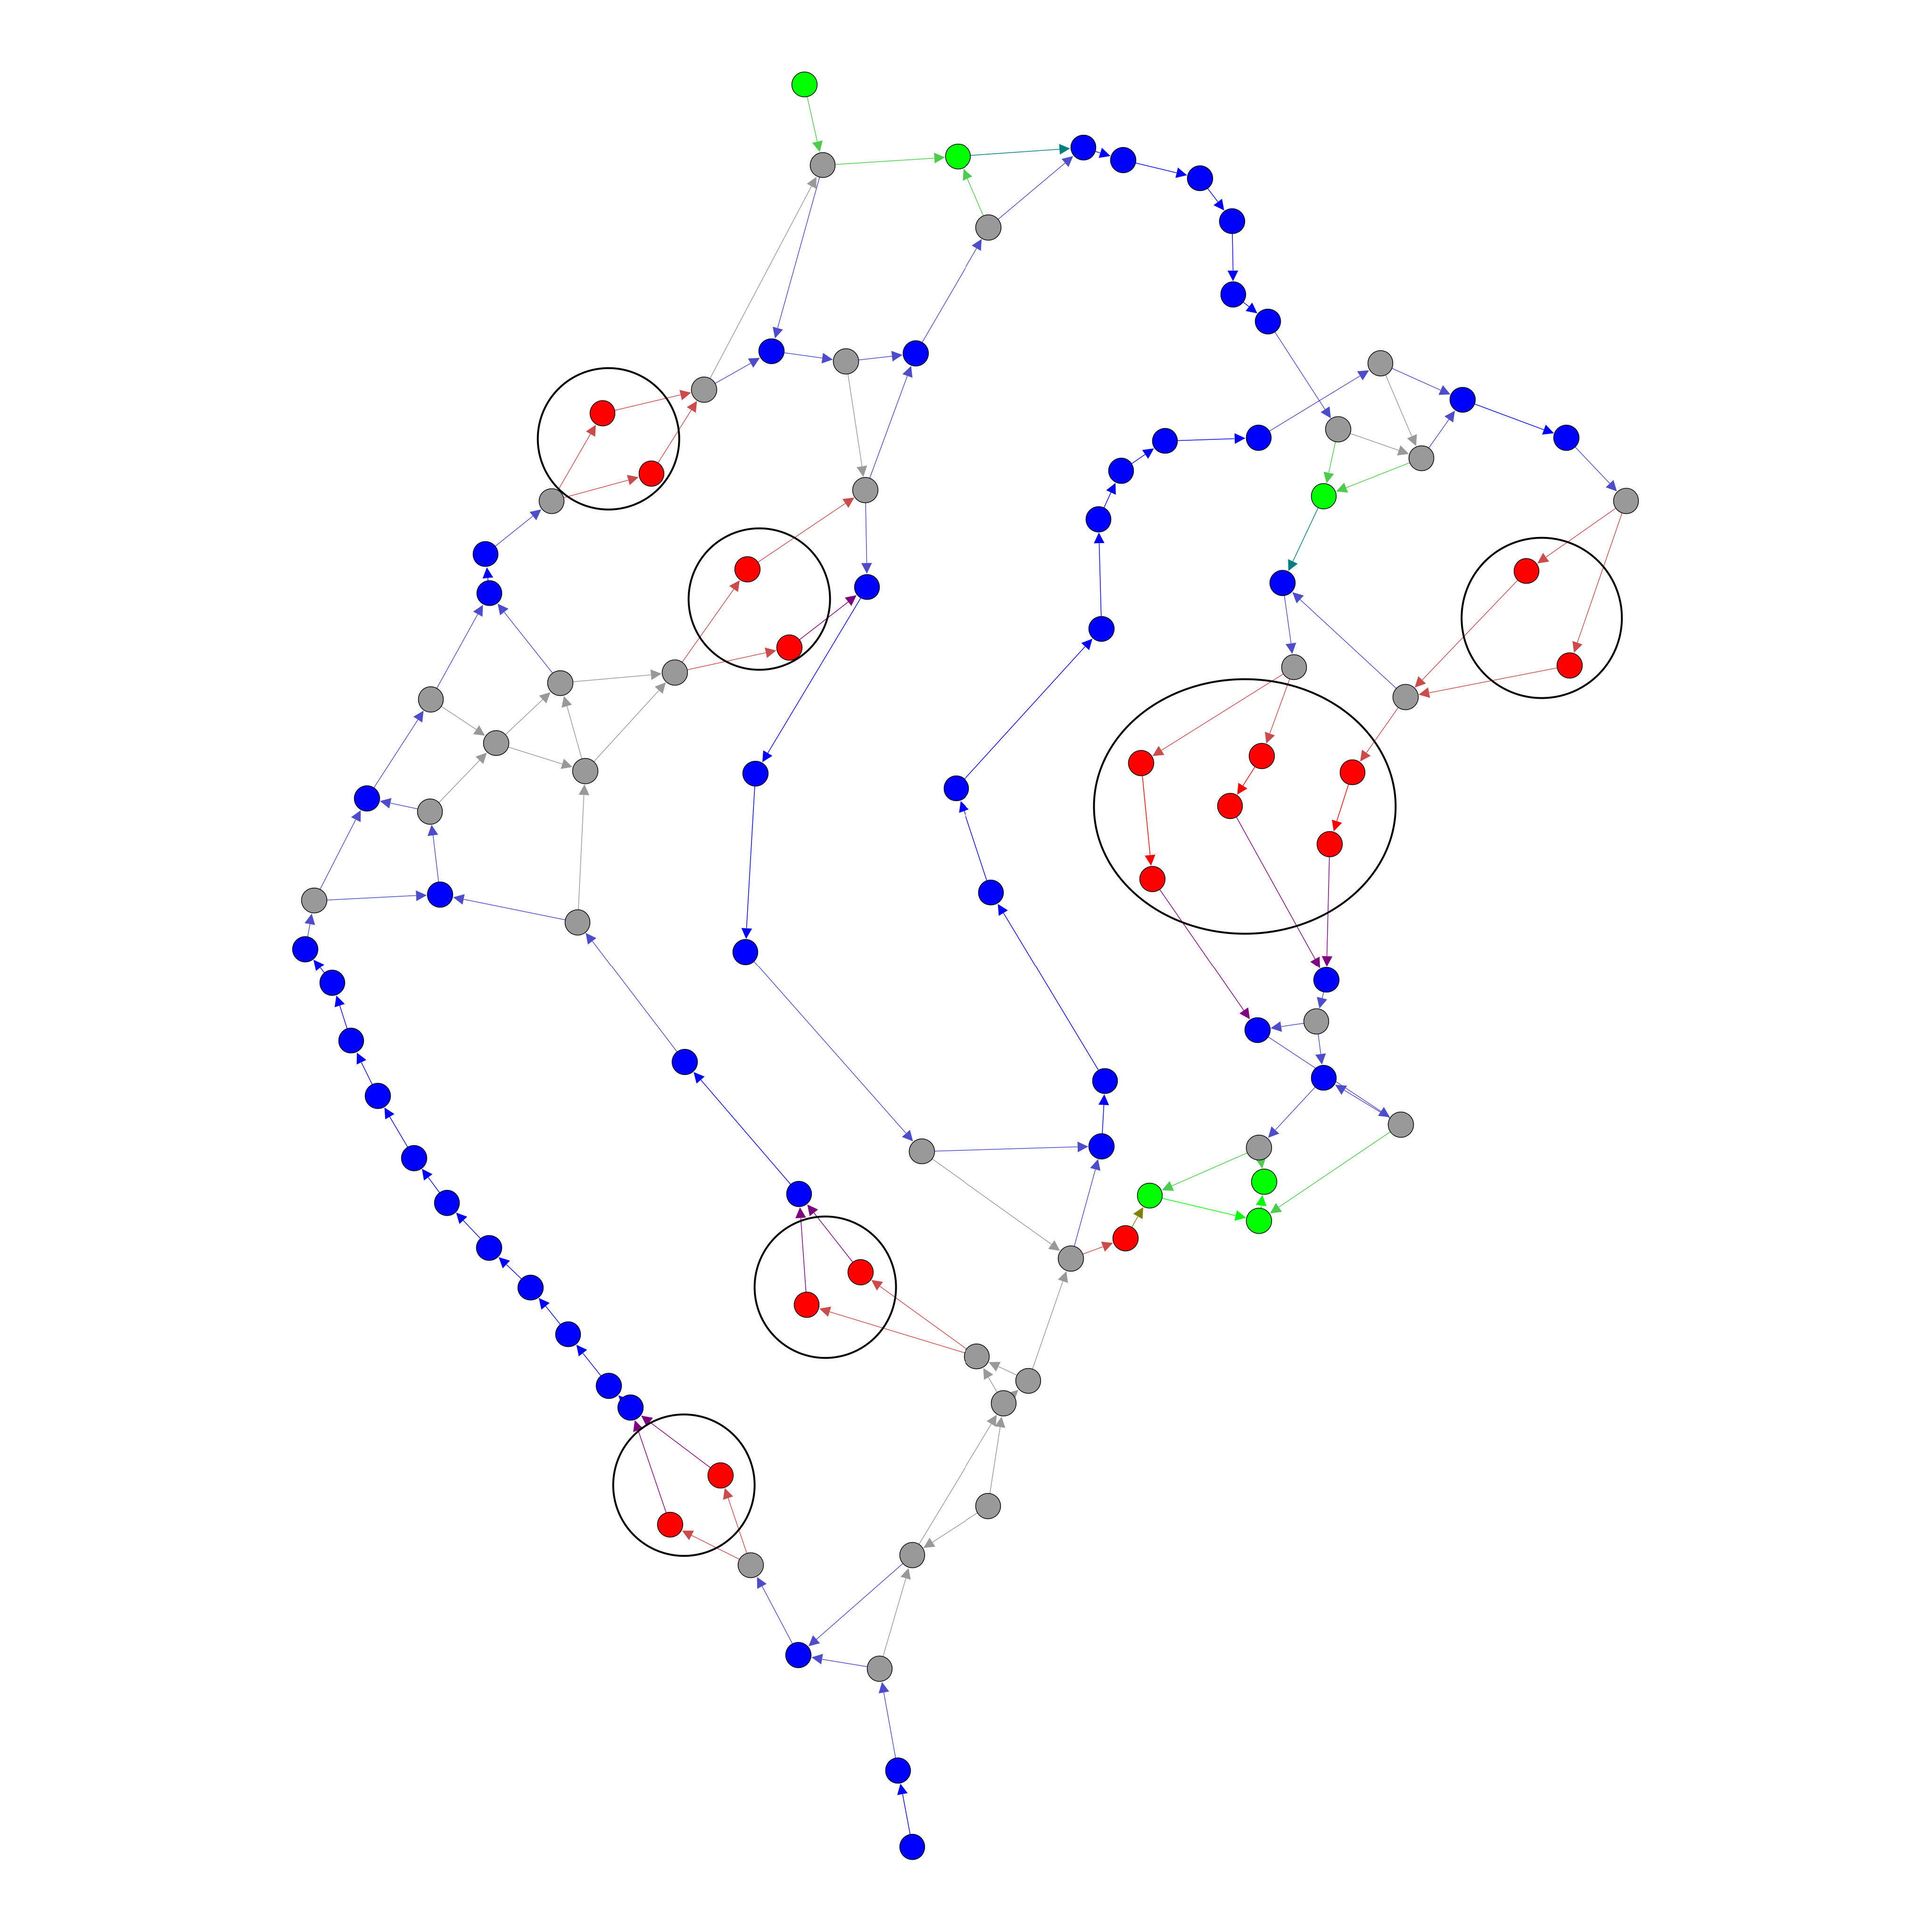
\includegraphics[scale=0.0375]{experimentation/deadlock/deadlock.png}}
	\caption{Potential deadlocks in MultiChain.}
	\label{fig:deadlock-double}
\end{figure}